


\documentclass[amssymb,twocolumn,aps]{revtex4}

%%%%%%%%%%%%%%%%%%%%%%%%%%%%%%%%%%%%%%%
%%%%%%%%%%%%%%% PACKAGES %%%%%%%%%%%%%%
%%%%%%%%%%%%%%%%%%%%%%%%%%%%%%%%%%%%%%%

\usepackage[utf8]{inputenc}
\usepackage[T1]{fontenc}
\usepackage[english]{babel}
\usepackage{lmodern}
\usepackage{mathtools,amssymb,bm,graphicx}
\usepackage{booktabs,array,dcolumn,siunitx}
\usepackage{float}
\usepackage{placeins}
\usepackage{enumitem}
\usepackage{nameref}
\usepackage{microtype}
\usepackage{hyperref}     
\usepackage{cleveref}      
\usepackage{algorithm}
\usepackage{algpseudocode}
\usepackage{url}
\usepackage{listings}
\usepackage{xcolor}
\usepackage{ragged2e}
\usepackage{etoolbox}
\usepackage{tabularx}
\usepackage{makecell}
\usepackage{setspace}
\usepackage{adjustbox}

%%%%%%%%%%%%%%%%%%%%%%%%%%%%%%%%%%%%%%%
%%%%%%%%%%% FIGURE CAPTIONS %%%%%%%%%%%
%%%%%%%%%%%%%%%%%%%%%%%%%%%%%%%%%%%%%%%
\makeatletter
\def\fnum@figure{\textbf{Figure~\thefigure}}
\makeatother
% \usepackage{subcaption}
% \usepackage{caption}
% \captionsetup{%
%   justification   = centerfirst, % Adjusted to center single-line captions and justify multi-line ones
%   singlelinecheck = false,
%   labelfont       = bf,
%   textfont        = small,
%   margin          = 6pt,
%   format          = plain,
%   skip            = 4pt
% }

%%%%%%%%%%%%%%%%%%%%%%%%%%%%%%%%%%%%%%%
%%%%%%%%%%% DISPLAY SPACING %%%%%%%%%%%
%%%%%%%%%%%%%%%%%%%%%%%%%%%%%%%%%%%%%%%

% tighten equation / align / align* spacing for revtex4
\makeatletter
\g@addto@macro\normalsize{%
  \setlength{\abovedisplayskip}{6pt}%
  \setlength{\belowdisplayskip}{6pt}%
  \setlength{\abovedisplayshortskip}{4pt}%
  \setlength{\belowdisplayshortskip}{4pt}%
}
\makeatother

%%%%%%%%%%%%%%%%%%%%%%%%%%%%%%%%%%%%%%%
%%%%%%%% REDUCE SECTION SPACING %%%%%%%
%%%%%%%%%%%%%%%%%%%%%%%%%%%%%%%%%%%%%%%

\preto{\section}{\vspace{-10pt}}
\preto{\subsection}{\vspace{-6pt}}
\preto{\subsubsection}{\vspace{-6pt}}
\setlength{\parskip}{0pt}
\setlength{\parindent}{15pt}

%%%%%%%%%%%%%%%%%%%%%%%%%%%%%%%%%%%%%%%
%%%%%%%%%%%% LISTINGS STYLE %%%%%%%%%%%
%%%%%%%%%%%%%%%%%%%%%%%%%%%%%%%%%%%%%%%

\definecolor{codebg}{RGB}{245,245,244}
\definecolor{codeframe}{RGB}{200,200,200}
\definecolor{codekeyword}{RGB}{0,0,180}
\definecolor{codestring}{RGB}{163,21,21}
\definecolor{codecomment}{RGB}{0,128,0}
\definecolor{codeidentifier}{RGB}{75,0,130}

\lstdefinestyle{pythonstyle}{
    language=Python,
    backgroundcolor=\color{codebg},
    frame=single,
    rulecolor=\color{codeframe},
    basicstyle=\ttfamily\small,
    keywordstyle=\color{codekeyword}\bfseries,
    stringstyle=\color{codestring},
    commentstyle=\color{codecomment}\itshape,
    identifierstyle=\color{codeidentifier},
    showstringspaces=false,
    breaklines=true,
    captionpos=b,
    tabsize=4,
    numbers=left,
    numbersep=6pt,
    numberstyle=\tiny\color{gray},
    framexleftmargin=6pt,
    framextopmargin=4pt,
    framexbottommargin=4pt,
    xleftmargin=10pt,
    xrightmargin=5pt
}

%%%%%%%%%%%%%%%%%%%%%%%%%%%%%%%%%%%%%%%
%%%%%%%%%%%% GENERAL SETTINGS %%%%%%%%%
%%%%%%%%%%%%%%%%%%%%%%%%%%%%%%%%%%%%%%%

\renewcommand{\refname}{\textbf{References}}
\crefname{lstlisting}{Listing}{Listings}
\Crefname{lstlisting}{Listing}{Listings}
\usepackage{microtype}
\microtypecontext{spacing=nonfrench}

%%%%%%%%%%%%%%%%%%%%%%%%%%%%%%%%%%%%%%%
%%%%%%%%%%%%%%%% DOCUMENT %%%%%%%%%%%%%
%%%%%%%%%%%%%%%%%%%%%%%%%%%%%%%%%%%%%%%

\begin{document}
\input{01 TITLE}
\onecolumngrid
\input{02 ABSTRACT}
\vspace{2em}
\twocolumngrid
\section{Introduction}\label{section:Introduction}

This is an intro lorem ipsum with a reference \textcite{hastie} and such \parencite{hastie}. 
\section{Methods}\label{section:methods}

\subsection{Methods used in Part A}

One-Qubit bases

\begin{equation}\label{single-qubits}
    \ket{0} = \begin{pmatrix}
        1\\0
    \end{pmatrix}\quad
    \ket{1} = \begin{pmatrix}
        0\\1
    \end{pmatrix}
\end{equation}

Pauli Matrices

\begin{equation}\label{pauli-matrices}
    \sigma_x=\begin{pmatrix}
        0&1\\1&0
    \end{pmatrix}\quad
    \sigma_y=\begin{pmatrix}
        0&-i\\i&0
    \end{pmatrix}\quad
    \sigma_z=\begin{pmatrix}
        1&0\\0&-1
    \end{pmatrix}
\end{equation}

Hadamard and Phase Gates

\begin{equation}
    H = \frac{1}{\sqrt{2}}\begin{pmatrix}
        1&1\\1&-1
    \end{pmatrix}\quad
    S = \begin{pmatrix}
        1&0\\0&-i
    \end{pmatrix}
\end{equation}

Kronecker products for basis states

\begin{equation}
\ket{00} = \ket{0} \otimes \ket{0}
\quad
\ket{01} = \ket{0} \otimes \ket{1}
\end{equation}

\begin{equation}
\ket{10} = \ket{1} \otimes \ket{0}
\quad
\ket{11} = \ket{1} \otimes \ket{1}
\end{equation}

Bell states

\begin{equation}
\ket{\Phi^+} = \frac{\ket{00} + \ket{11}}{\sqrt{2}}
\quad
\ket{\Phi^-} = \frac{\ket{00} - \ket{11}}{\sqrt{2}}
\end{equation}

\begin{equation}
\ket{\Psi^+} = \frac{\ket{01} + \ket{10}}{\sqrt{2}}
\quad
\ket{\Psi^-} = \frac{\ket{01} - \ket{10}}{\sqrt{2}}
\end{equation}

\begin{equation}
    \text{CNOT} = \begin{pmatrix}
        1&0&0&0\\
        0&1&0&0\\
        0&0&0&1\\
        0&0&1&0
    \end{pmatrix}
\end{equation}



\subsection{Methods used in Part B}

We define a symmetric matrix $H\in\mathbb{R}^{2\times2}$

\begin{equation}
    H=\begin{bmatrix}
        H_{11} & H_{12} \\
        H_{21} & H_{22}
    \end{bmatrix}
\end{equation}

We let $H=H_0+H_1$ where

\begin{equation}
    H_0=\begin{bmatrix}
        E_1 & 0 \\
        0 & E_2
    \end{bmatrix}
\end{equation}

is a diagonal matrix.

Similarly,

\begin{equation}
    H_1=\begin{bmatrix}
        V_{11} & V_{12} \\
        V_{21} & V_{22}
    \end{bmatrix}
\end{equation}

Where $V_{ij}$ represents various interaction matrix elements. We can view $H_0$ as the non-interacting solution

\begin{equation}
    H_0\ket{0} = E_1\ket{0}
\end{equation}

\begin{equation}
    H_0\ket{1}=E_2\ket{1}
\end{equation}

We rewrite $H$ with $H_0$ and $H_1$ via Pauli matrices

\begin{equation}
    H_0=\mathcal{E}I+\Omega\sigma_Z
\end{equation}

\begin{equation}
    \mathcal{E} = \frac{E_1+E_2}{2}
\end{equation}

\begin{equation}
    \Omega=\frac{E_1-E_2}{2}
\end{equation}

\begin{equation}
    H_I=c\textbf{I}+\omega_z\sigma_z+\omega_x\sigma_x
\end{equation}

\begin{equation}
    c=\frac{V_{11}+V_{22}}{2}
\end{equation}

\begin{equation}
    \omega_z=\frac{V_{11}-V_{22}}{2}
\end{equation}

\begin{equation}
    \omega_x=V_{12}=V_{21}
\end{equation}

We let our Hamiltonian depend linearly on a strenght parameter $\lambda$

\begin{equation}
    H=H_0+\lambda H_1
\end{equation}

with $\lambda\in[0,1]$ and limits $\lambda=0$, $\lambda=1$.

\subsection{Methods used in Part C}

\subsection{Methods used in Part D}

\subsection{Methods used in Part E}

\subsection{Methods used in Part F}

$H=H_0+H_1+H_2$

\begin{equation}
    H_0=\frac{1}{2}\varepsilon\sum_{p\sigma}\sigma a_{p\sigma}^{\dagger}a_{p\sigma}
\end{equation}

\begin{equation}
    H_1=\frac{1}{2}V\sum_{p,p',\sigma}\sigma a_{p\sigma}^{\dagger}a_{p\sigma}
\end{equation}

\begin{equation}
    H_2=\frac{1}{2}W\sum_{p,p',\sigma}a_{p\sigma}^{\dagger}a_{p'\sigma}^{\dagger}a_{p'-\sigma}a_{p-\sigma}
\end{equation}

\begin{equation}
    H_0=\varepsilon J_z
\end{equation}

\begin{equation}
    H_1=\frac{1}{2}V(J_+^2+J_-^2)
\end{equation}

\begin{equation}
    H_2=\frac{1}{2}W(-N+J_+J_-+J_-J_+)
\end{equation}

\begin{equation}
    H_{J=1} = \begin{pmatrix}
        -\epsilon & 0 & -V \\
        0 & 0 & 0 \\
        -V & 0 & \epsilon
    \end{pmatrix}
\end{equation}

For $J=2$ we have a $5\times5$ matrix given by

\begin{equation}
    H_{J=2}=\begin{pmatrix}
        -2\epsilon & 0 & \sqrt{6}V & 0 & 0 \\
        0 & -\epsilon + 3W  & 0 & 3V & 0 \\
        \sqrt{6}V & 0 & 4W & 0 & \sqrt{6}V \\
        0 & 3V & 0 & \epsilon+3W & 0 \\
        0 & 0& \sqrt{6}V & 0 & 2\varepsilon
    \end{pmatrix}
\end{equation}

\subsection{Methods used in Part G}
\section{Results}\label{section:result}

\subsection{Part A results}

\subsection{Part B results}

\begin{lstlisting}[caption={VQE solver loop},label={lst:vqe-loop}]
# Solve for lambda in [0, 1]
lambdas = np.linspace(0, 1, 101)
eigvals = []
eigvecs = []

for l in lambdas:
    H = H0 + l * HI
    w, v = np.linalg.eigh(H)
    eigvals.append(w)
    eigvecs.append(v)

eigvals = np.array(eigvals)
eigvecs = np.array(eigvecs)
\end{lstlisting}

\subsection{Part C results}

\begin{equation}
    E_1=0.0
    \quad
    E_2 = 4.0
\end{equation}
\begin{equation}
    V_{11} = 3.0 \quad V_{12} = 0.2
\end{equation}
\begin{equation}
    V_{21} = 0.2 \quad V_{22} = -3.0
\end{equation}
\begin{equation}
    H_0=\begin{pmatrix}
        E_1&0\\0&E_2
    \end{pmatrix}
    =\begin{pmatrix}
        0&0\\0&4
    \end{pmatrix}
\end{equation}
\begin{equation}
    H_I = \begin{pmatrix}
        V_{11} & V_{12} \\
        V_{21} & V_{22}
    \end{pmatrix}
    =\begin{pmatrix}
        3.0 & 0.2 \\
        0.2 & -3.0
    \end{pmatrix}
\end{equation}

\begin{equation}
    \mathcal{E} = 2.0 \quad \Omega=-2.0 \quad \omega_z=3.0 \quad \omega_x=0.2
\end{equation}

\begin{equation}
    H(\lambda)=H_0+\lambda H_1
\end{equation}

\begin{equation}
    H(\lambda)\mathbf{v}_i=E_i(\lambda)\mathbf{v}_i
\end{equation}

\begin{equation}
    H(\lambda)=\varepsilon\textbf{I}+(\lambda\omega_z+\Omega)\sigma_z+(\lambda\omega_x)\sigma_x
\end{equation}

\begin{equation}
    \ket{\psi(\theta)} = R_y(\theta)\ket{0}
\end{equation}

\begin{equation}
    \ket{\psi(\theta)} = \begin{pmatrix}
        \cos\left(\frac{\theta}{2}\right) \\ \sin\left(\frac{\theta}{2}\right)
    \end{pmatrix}
\end{equation}

\begin{equation}
    \langle\sigma_z\rangle=\cos(\theta) 
    \quad
    \langle\sigma_x\rangle=\sin(\theta)
\end{equation}

\begin{equation}
    E(\theta,\lambda) = \varepsilon+(\lambda\omega_z+\Omega)\cos(\theta)+(\lambda\omega_x)\sin(\theta)
\end{equation}

\begin{equation}
    E_{\text{VQE}}(\lambda)=\min_{\theta}E(\theta,\lambda)
\end{equation}
\begin{equation}
    E_{\text{exact}}(\lambda)
\end{equation}

\begin{equation}
    \lambda_i\in[0,1] \quad i=1,\dots,51 
\end{equation}

\subsection{Part D results}

\begin{equation}
    H_x=2.0 \quad H_z=3.0
\end{equation}

\begin{equation}
    \ket{\epsilon}_{00} = 0.0 \quad \ket{\epsilon}_{10} = 2.5
\end{equation}
\begin{equation}
    \ket{\epsilon}_{01} = 6.5 \quad \ket{\epsilon}_{11} = 7.0
\end{equation}


\subsection{Part E results}
\subsection{Part F results}
\subsection{Part G results}

\section{Conclusion}\label{section:conclusion}



\subsection{Sample-text}

Quantum computing builds on fundamental principles of quantum mechanics such as
superposition, interference, and entanglement, concepts that were already central
to early discussions about the completeness of quantum theory
\parencite{einstein_podolsky_rosen_1935}. Modern treatments of quantum computation
are typically grounded in the formal framework presented by
\textcite{nielsen_chuang_2000}, while more accessible introductions can be found
in texts such as \textcite{rieffel_polak_2011} and in pedagogical overviews aimed
at non-physicists \parencite{rieffel_intro_qc_nonphys_2000}. From a mathematical
perspective, the structure of quantum algorithms and Hilbert space methods is
explored in detail by \textcite{scherer_math_qc}, with complementary textbook
treatments provided in alternative presentations of the quantum information
framework \parencite{michaelsen_isaac_qci}. 

Within this broader landscape, the emerging field of quantum machine learning
(QML) seeks to combine ideas from classical statistical learning with quantum
algorithms. Classical foundations for statistical learning theory and modern
machine learning methods are well established in works such as
\textcite{hastie}, which provide the theoretical backbone for many learning
algorithms. Building on these principles, several authors have developed
dedicated treatments of QML, including comprehensive overviews
\parencite{conti_qml, schuld_qml} and more practical programming-oriented
introductions \parencite{pattanayak_qml_python}. Current algorithmic research
often focuses on hybrid quantum–classical methods designed for near-term
quantum devices. For instance, the Variational Quantum Eigensolver (VQE) has
emerged as one of the most widely studied approaches for optimization and
quantum simulation problems, with extensive methodological surveys available
in the literature \parencite{tilly_vqe_review_2022}. Closely related ideas appear
in the Quantum Approximate Optimization Algorithm (QAOA), whose theoretical
performance and practical implementation on near-term hardware have recently
been analyzed in detail \parencite{zhou_qaoa_perf_2025}, with introductory
expositions available in recent tutorial-style papers
\parencite{giovagnoli_qoao_intro}. 

In addition to traditional academic literature, open educational resources and
code repositories have become an important part of the quantum computing
ecosystem. For example, the publicly available course repository by
\textcite{compphysics_qcml_2026} provides practical implementations and teaching
material covering both quantum algorithms and quantum machine learning methods.
\clearpage
\onecolumngrid
\section{Appendix}\label{section:appendix}

% ---------------- Part A ----------------
\begin{figure}[H]
    \centering
    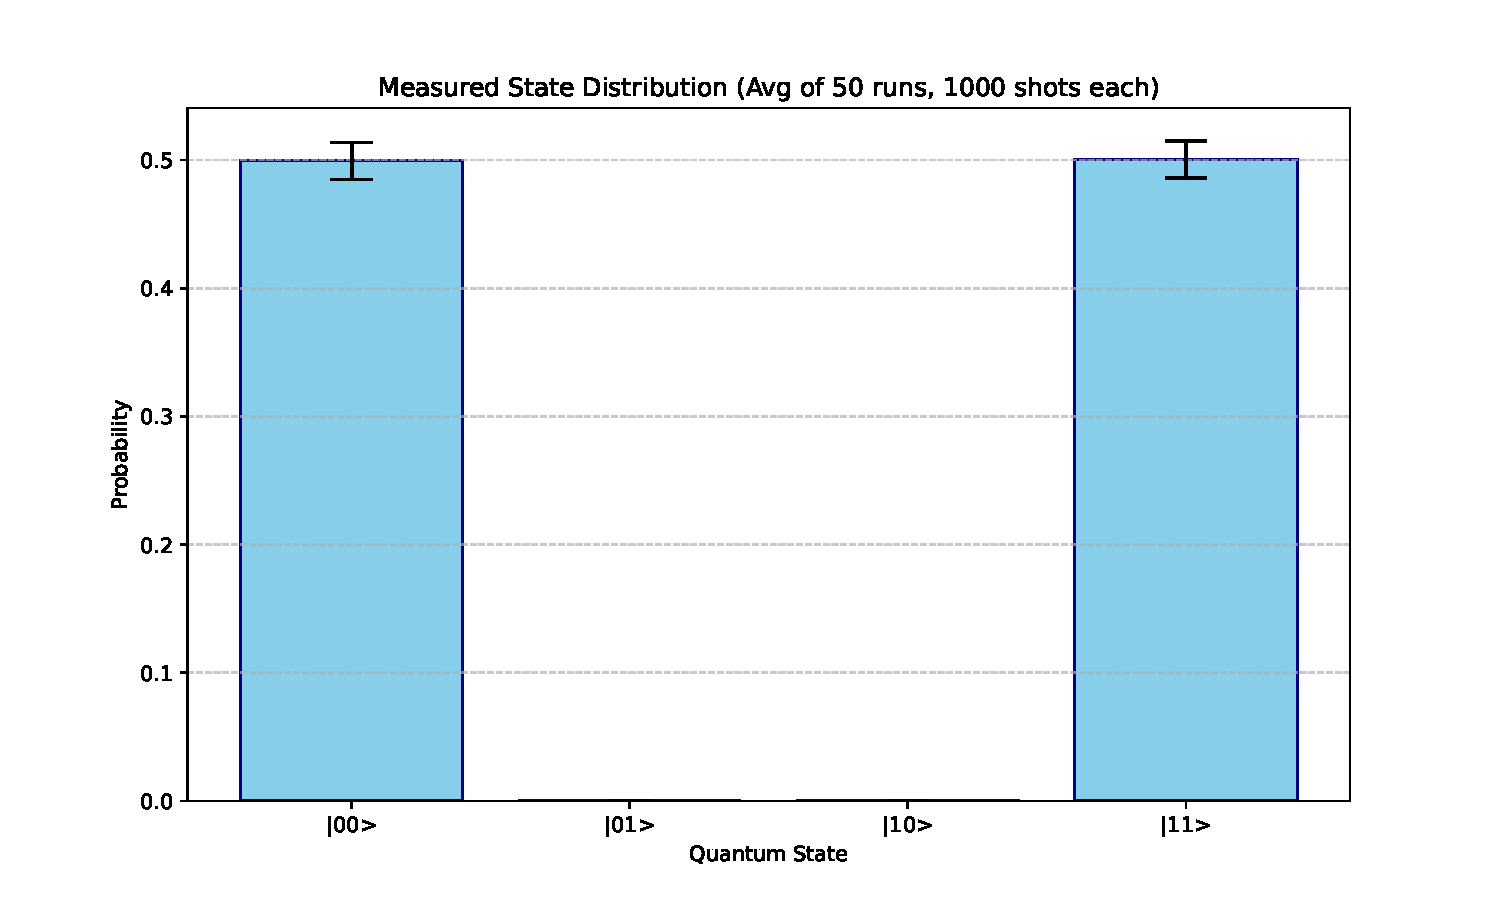
\includegraphics[width=0.55\linewidth]{figures/part-a_measurement_dist.pdf}
    \caption{Measurement distribution (Part A).}
    \label{fig:parta_measurement_distribution}
\end{figure}

% ---------------- Part B ----------------
\begin{figure}[H]
    \centering
    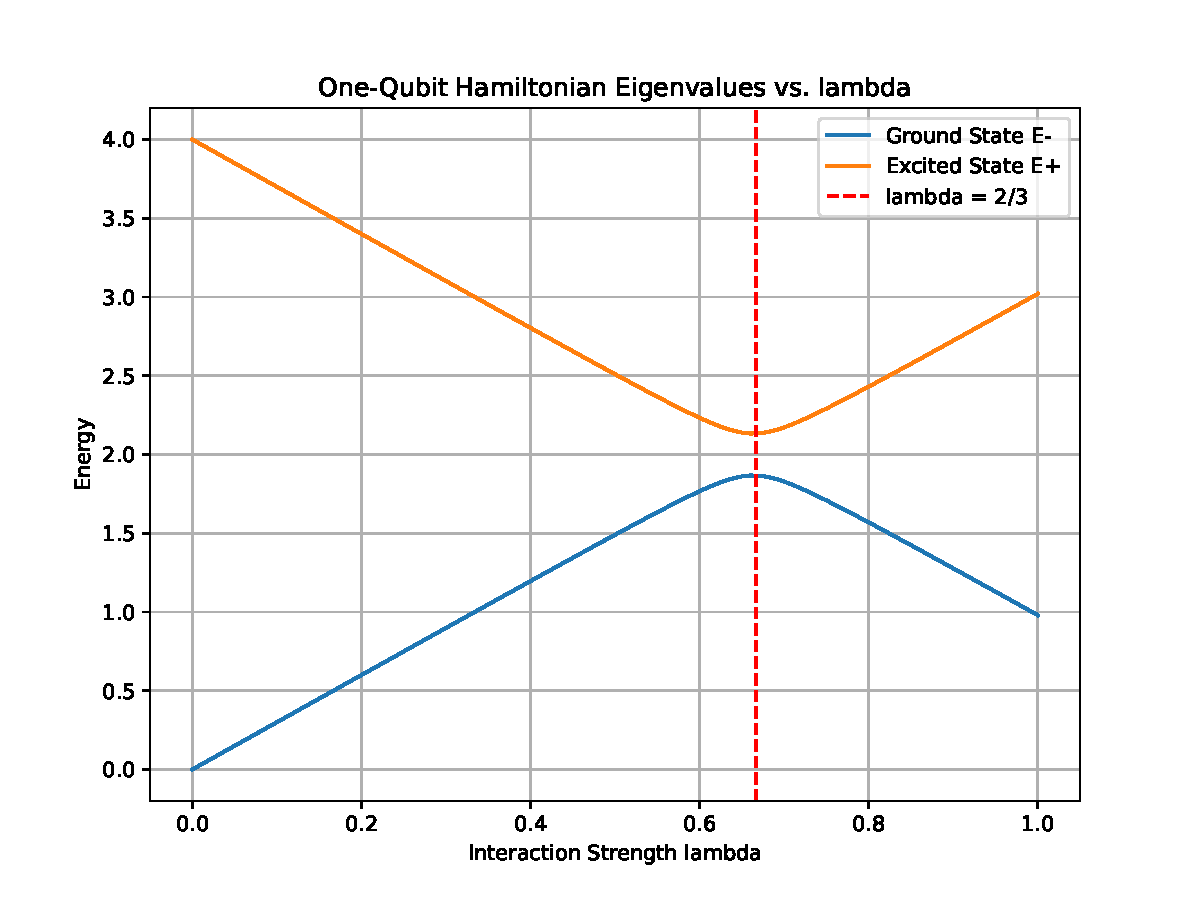
\includegraphics[width=0.55\linewidth]{figures/part-b_eigenvalues.pdf}
    \caption{Eigenvalue spectrum of the Hamiltonian (Part B).}
    \label{fig:partb_eigenvalues}
\end{figure}

\begin{figure}[H]
    \centering
    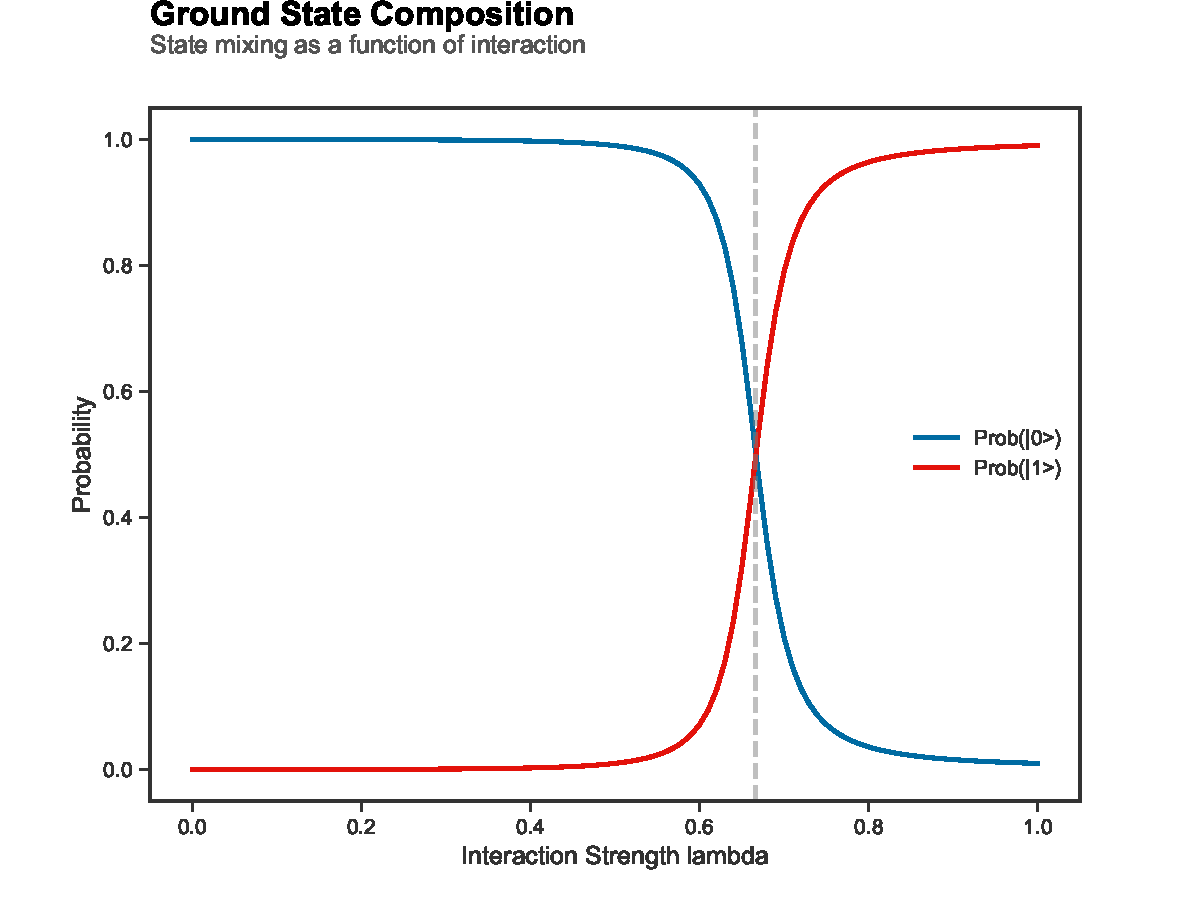
\includegraphics[width=0.55\linewidth]{figures/part-b_eigenvector_mixing.pdf}
    \caption{Eigenvector mixing across the spectrum (Part B).}
    \label{fig:partb_eigenvector_mixing}
\end{figure}

% ---------------- Part C ----------------
\begin{figure}[H]
    \centering
    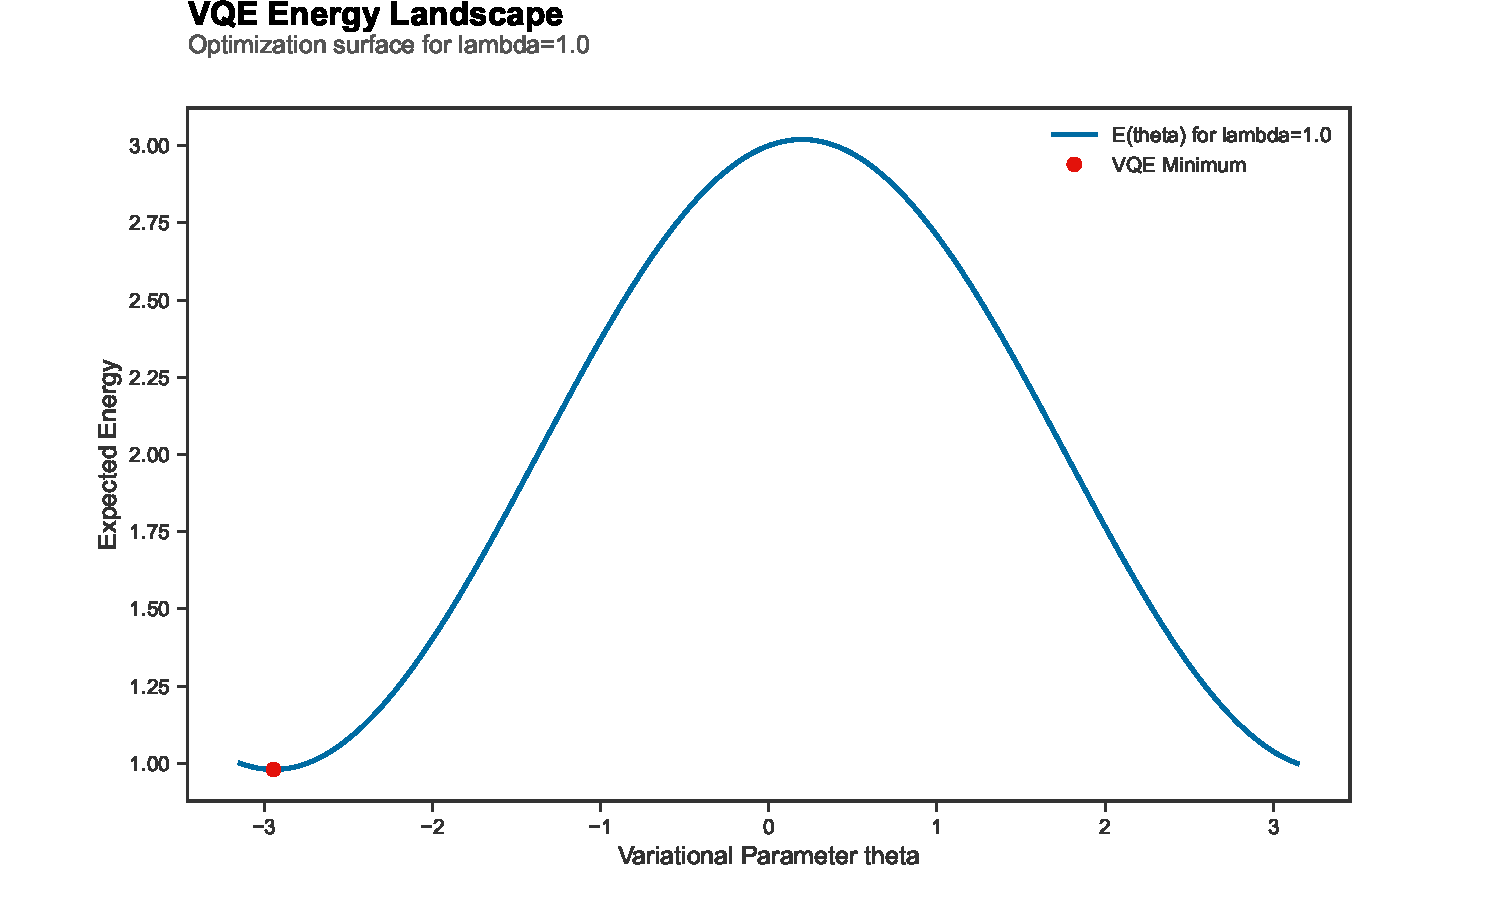
\includegraphics[width=0.55\linewidth]{figures/part-c_energy_landscape.pdf}
    \caption{Energy landscape over the variational parameter space (Part C).}
    \label{fig:partc_energy_landscape}
\end{figure}

\begin{figure}[H]
    \centering
    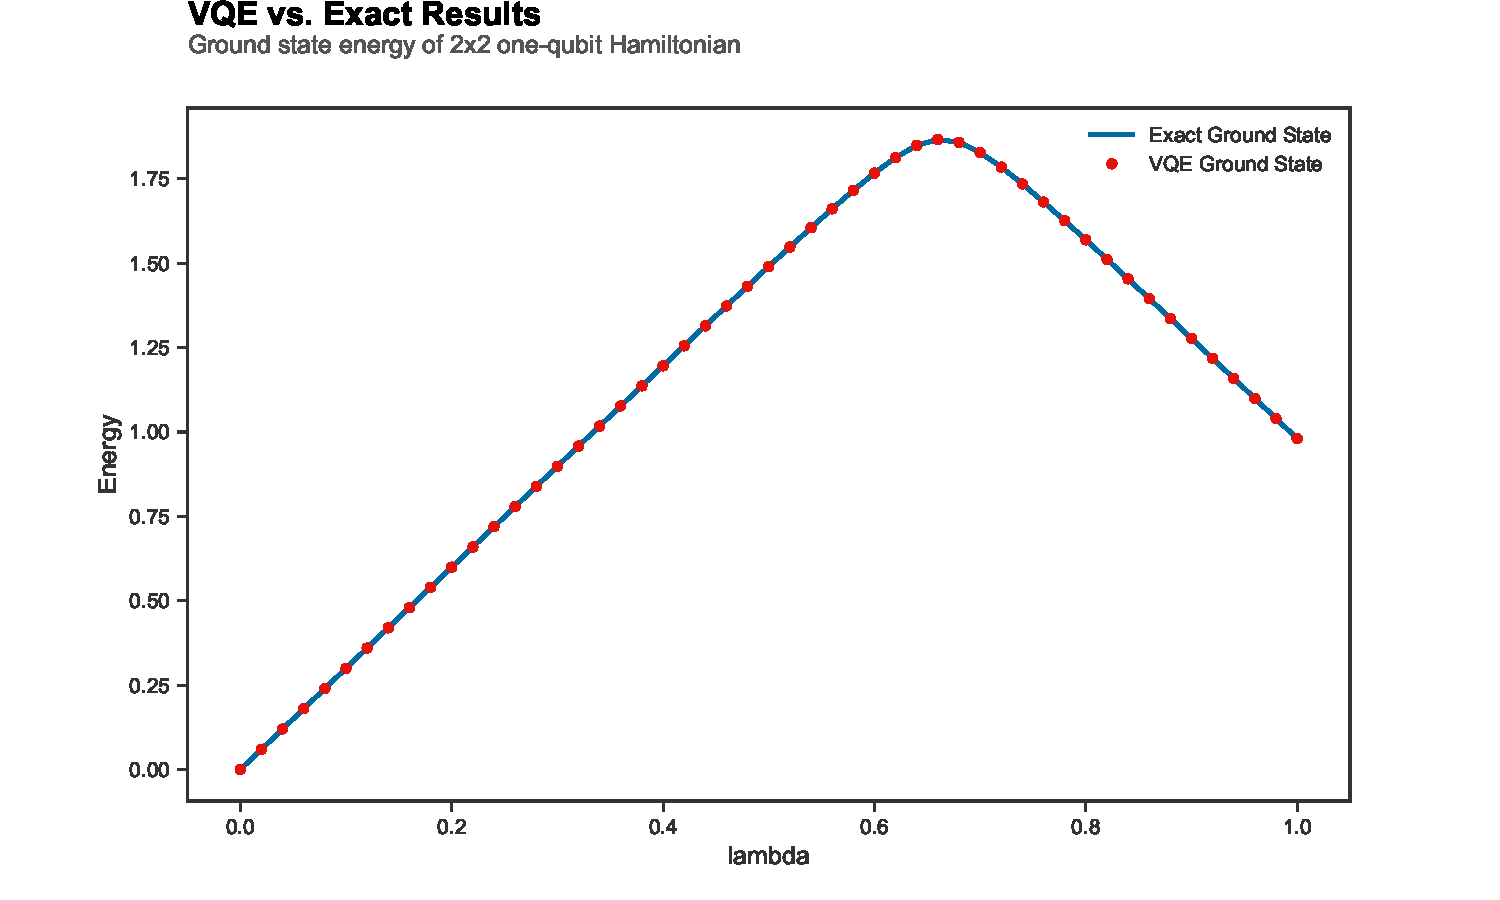
\includegraphics[width=0.55\linewidth]{figures/part-c_vqe_comp.pdf}
    \caption{VQE energy convergence compared to the exact ground-state energy (Part C).}
    \label{fig:partc_vqe_comparison}
\end{figure}

\begin{figure}[H]
    \centering
    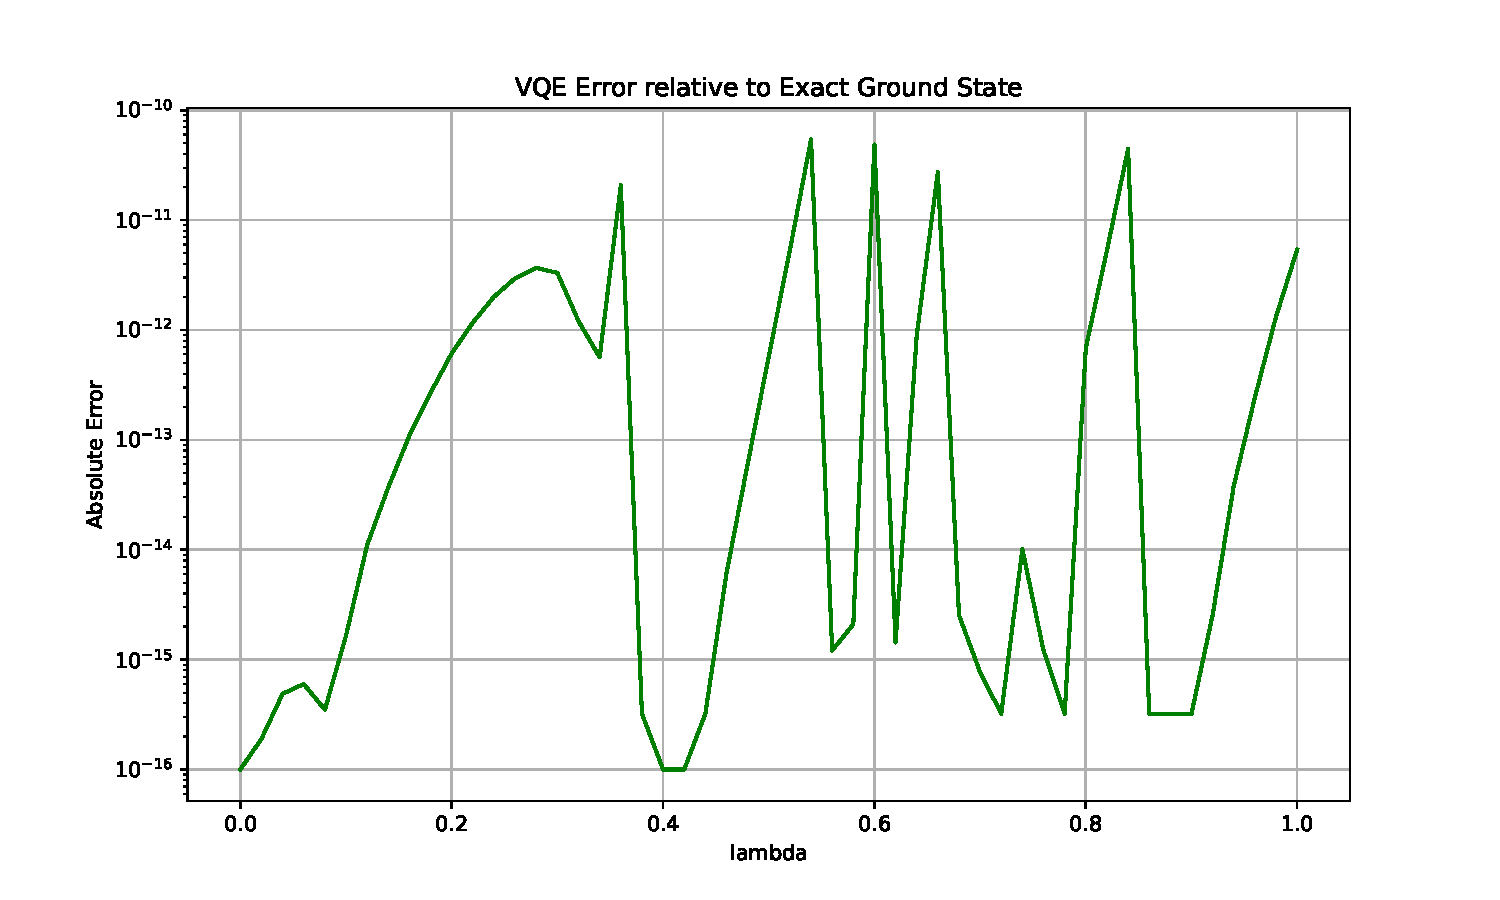
\includegraphics[width=0.55\linewidth]{figures/part-c_vqe_error.pdf}
    \caption{Absolute VQE error as a function of optimization iterations (Part C).}
    \label{fig:partc_vqe_error}
\end{figure}

% ---------------- Part D ----------------
\begin{figure}[H]
    \centering
    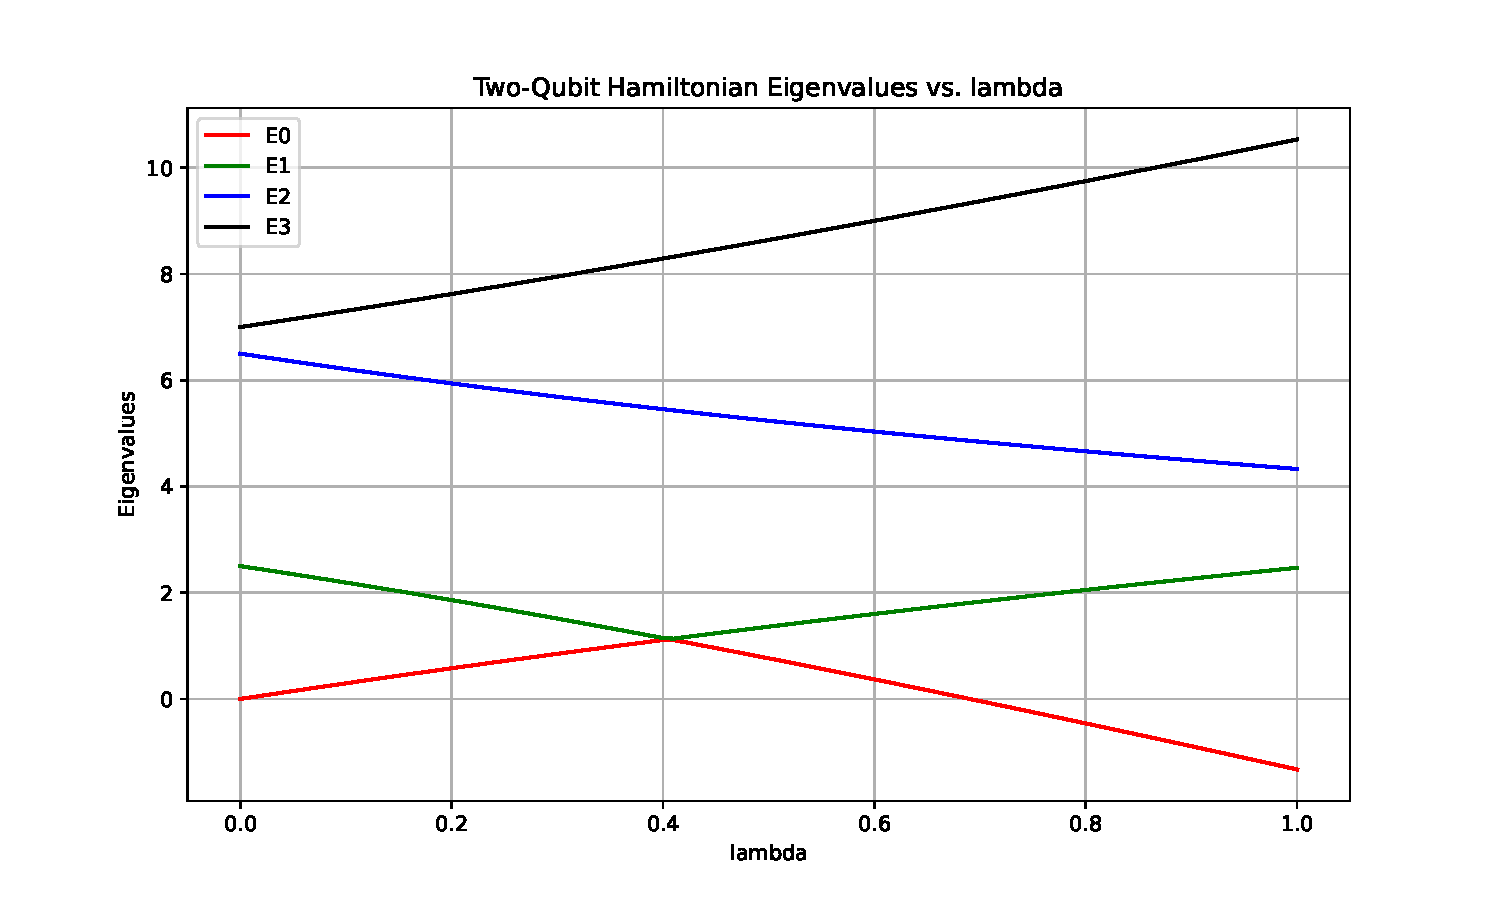
\includegraphics[width=0.55\linewidth]{figures/part-d_eigenvalues.pdf}
    \caption{Eigenvalue spectrum of the extended system (Part D).}
    \label{fig:partd_eigenvalues}
\end{figure}

\begin{figure}[H]
    \centering
    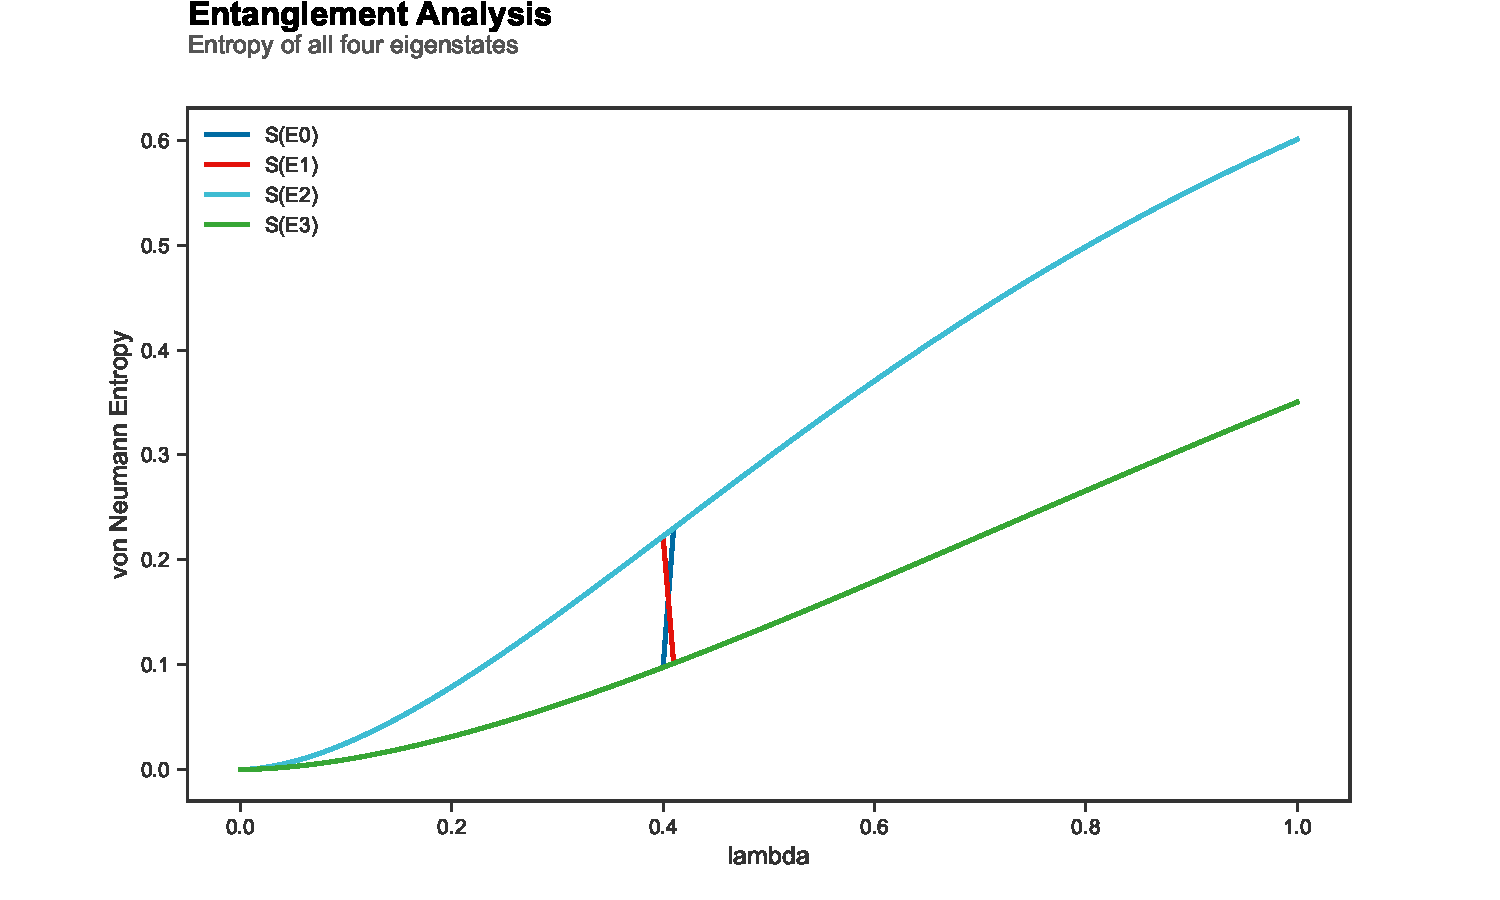
\includegraphics[width=0.55\linewidth]{figures/part-d_entropy.pdf}
    \caption{Bipartite entanglement entropy across system partitions (Part D).}
    \label{fig:partd_entropy}
\end{figure}

% ---------------- Part E ----------------
\begin{figure}[H]
    \centering
    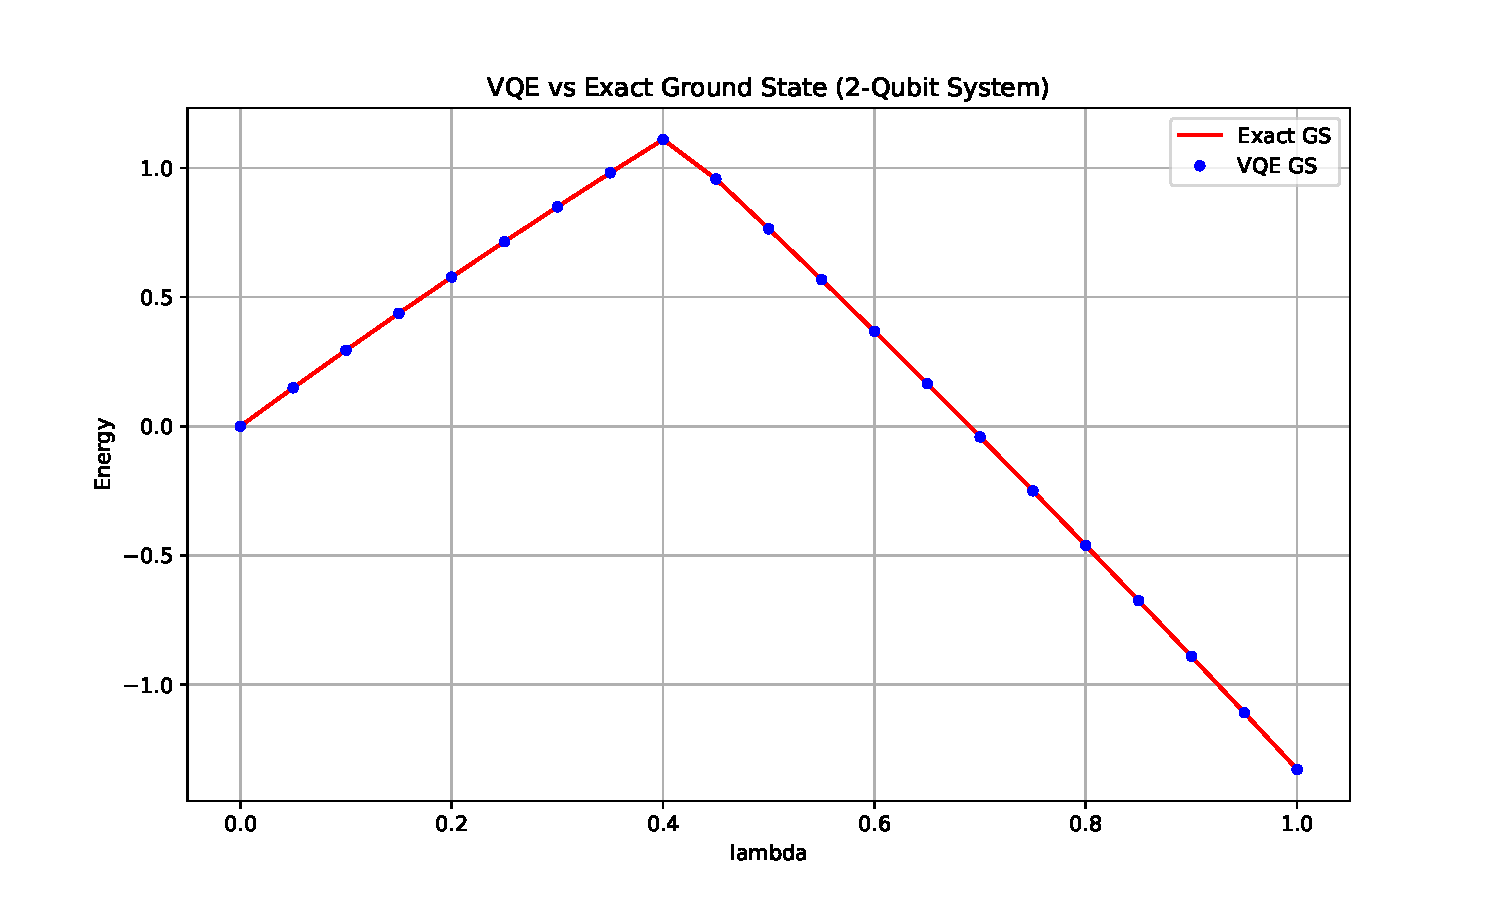
\includegraphics[width=0.55\linewidth]{figures/part-e_vqe_comp.pdf}
    \caption{VQE energy convergence for the modified Hamiltonian (Part E).}
    \label{fig:parte_vqe}
\end{figure}

% ---------------- Part F ----------------
\begin{figure}[H]
    \centering
    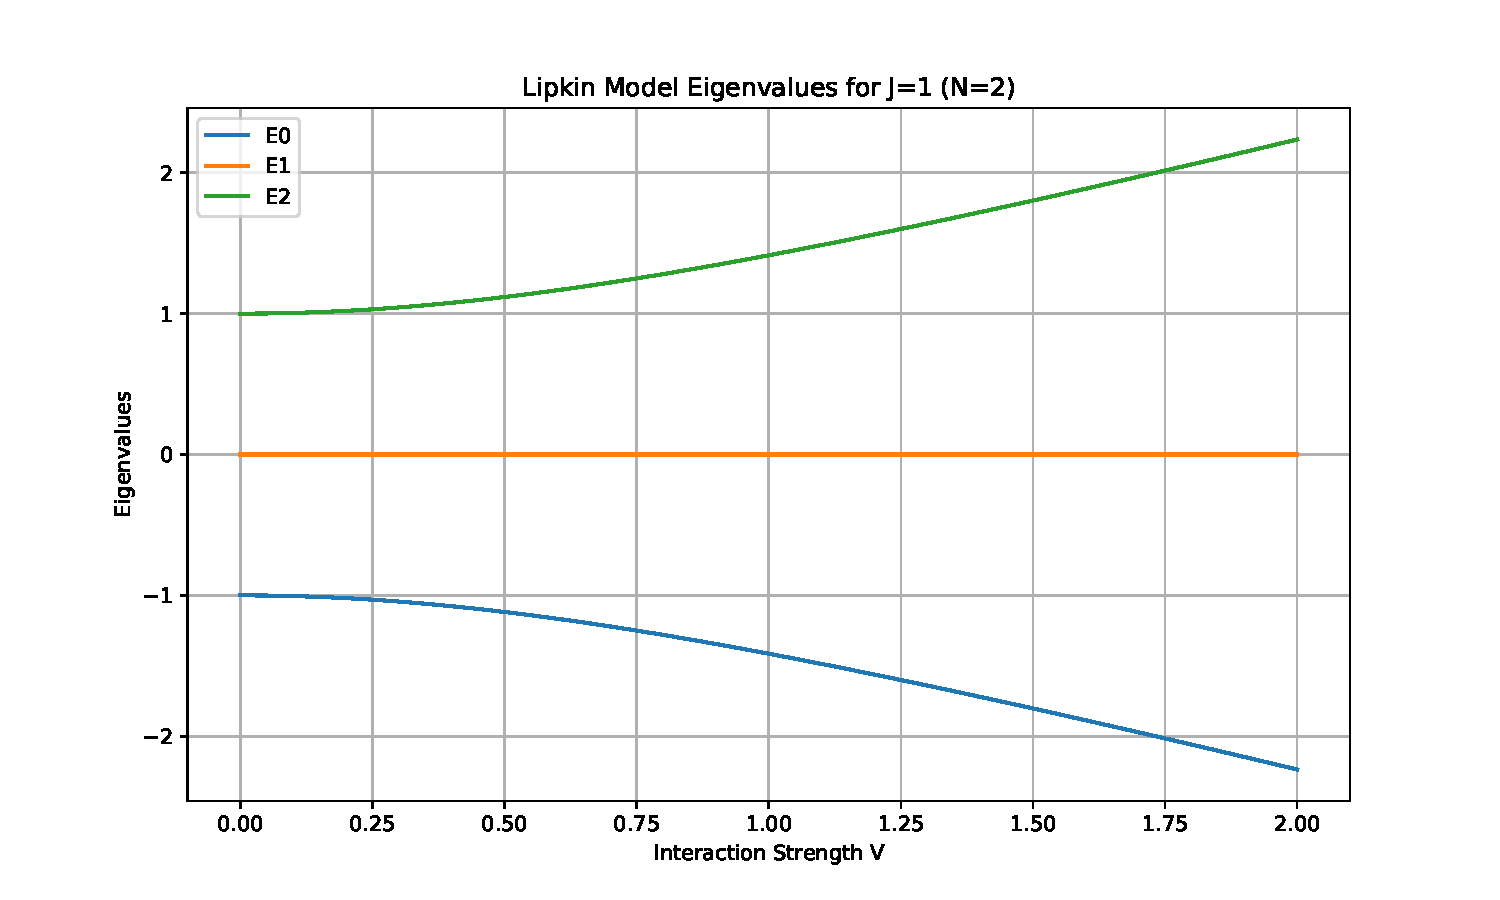
\includegraphics[width=0.55\linewidth]{figures/part-f_j1.pdf}
    \caption{Ground-state energy as a function of coupling parameter $J_1$ (Part F).}
    \label{fig:partf_j1}
\end{figure}

\begin{figure}[H]
    \centering
    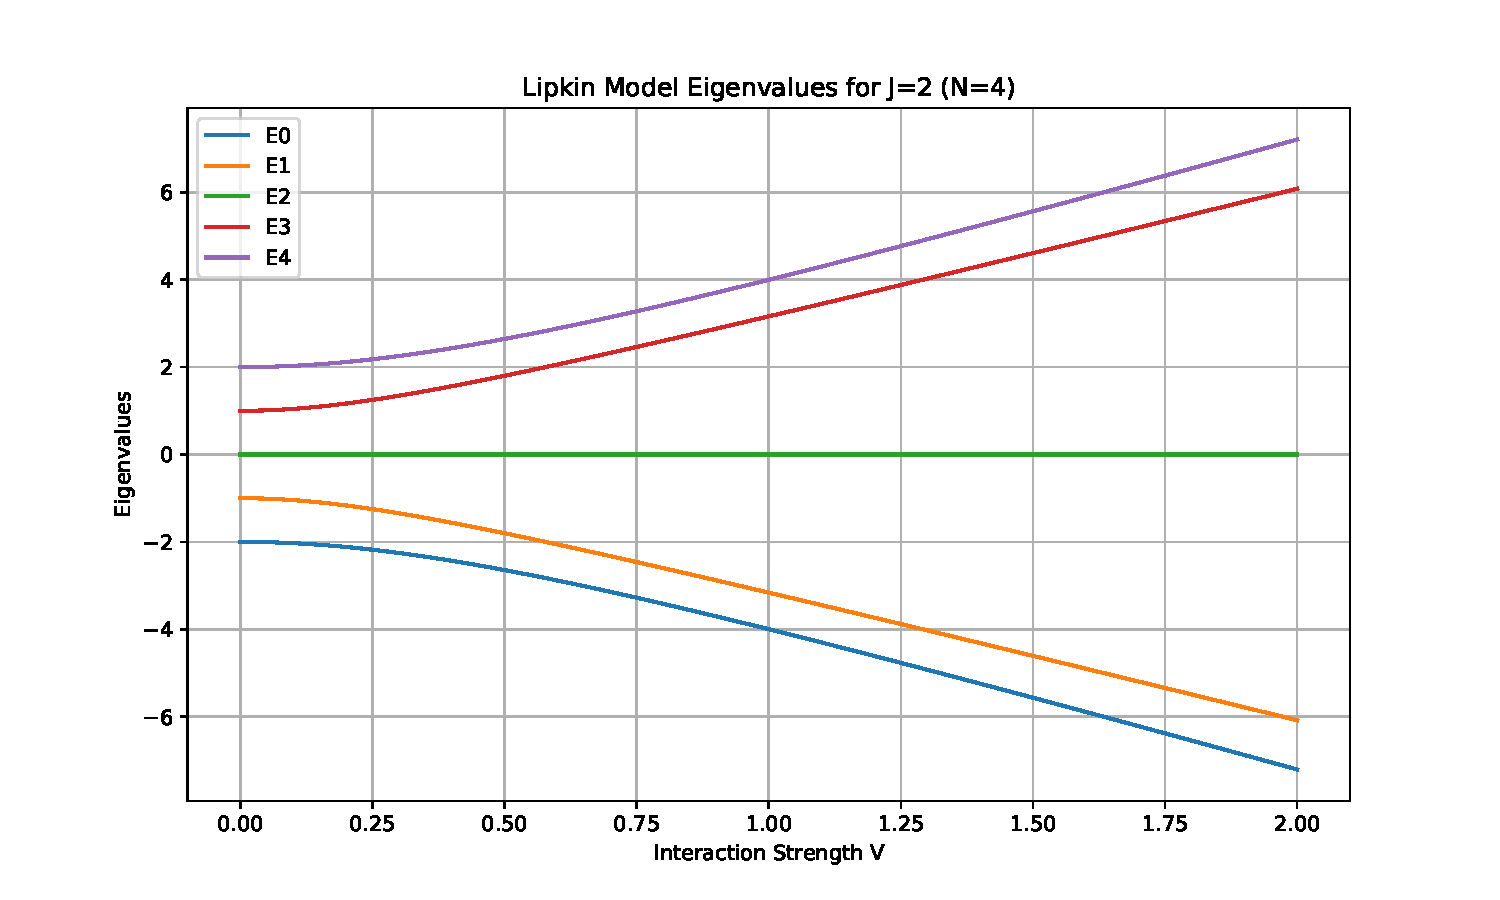
\includegraphics[width=0.55\linewidth]{figures/part-f_j2.pdf}
    \caption{Ground-state energy as a function of coupling parameter $J_2$ (Part F).}
    \label{fig:partf_j2}
\end{figure}

\begin{figure}[H]
    \centering
    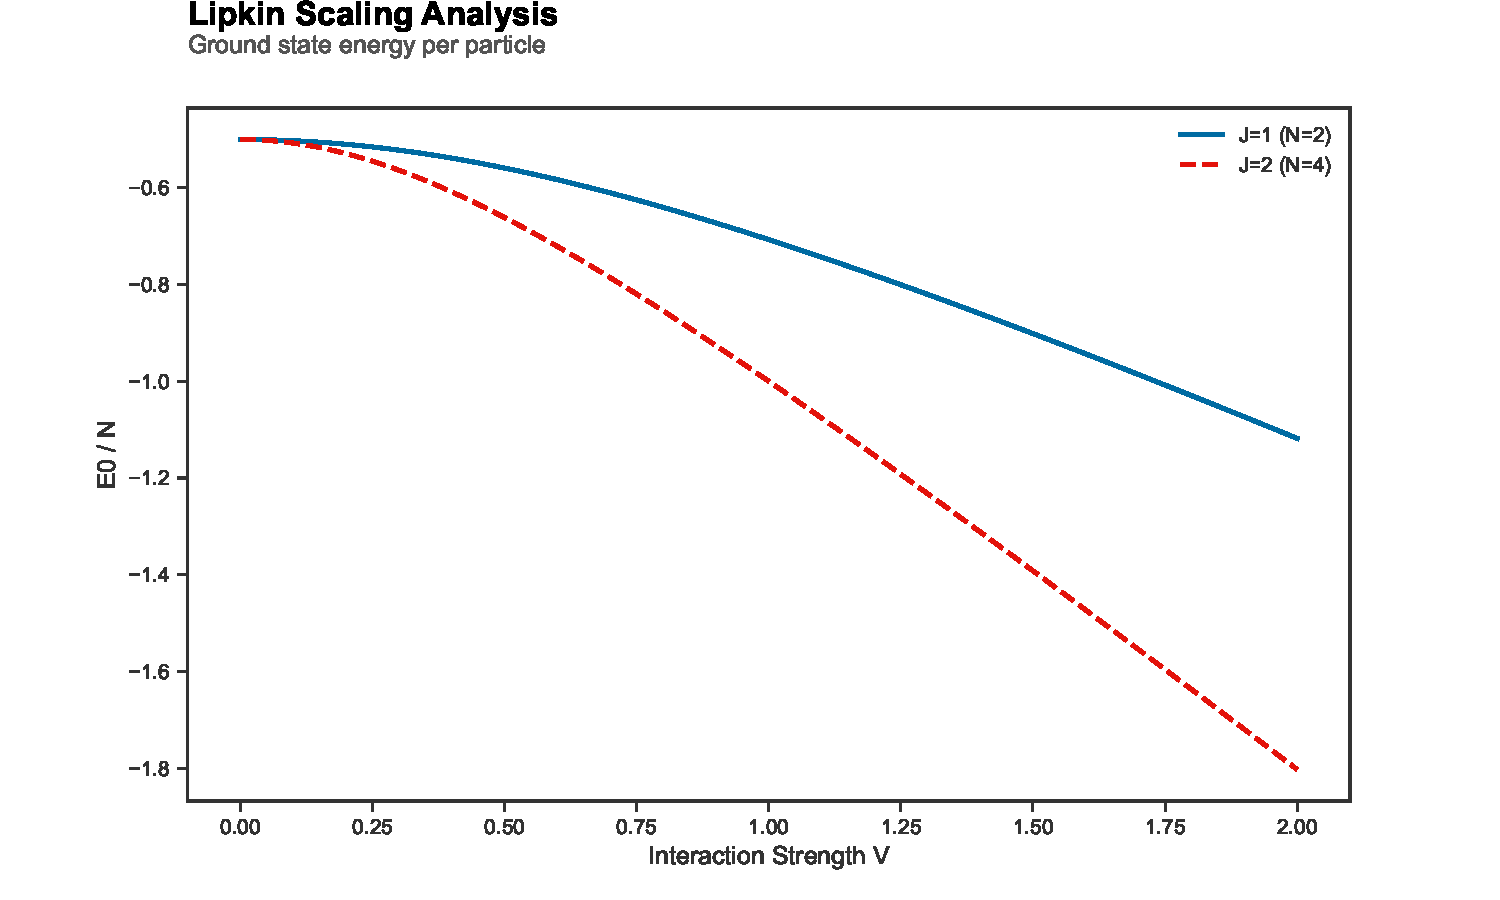
\includegraphics[width=0.55\linewidth]{figures/part-f_scaling.pdf}
    \caption{Scaling behavior of the ground-state energy with system size (Part F).}
    \label{fig:partf_scaling}
\end{figure}

% ---------------- Part G ----------------
\begin{figure}[H]
    \centering
    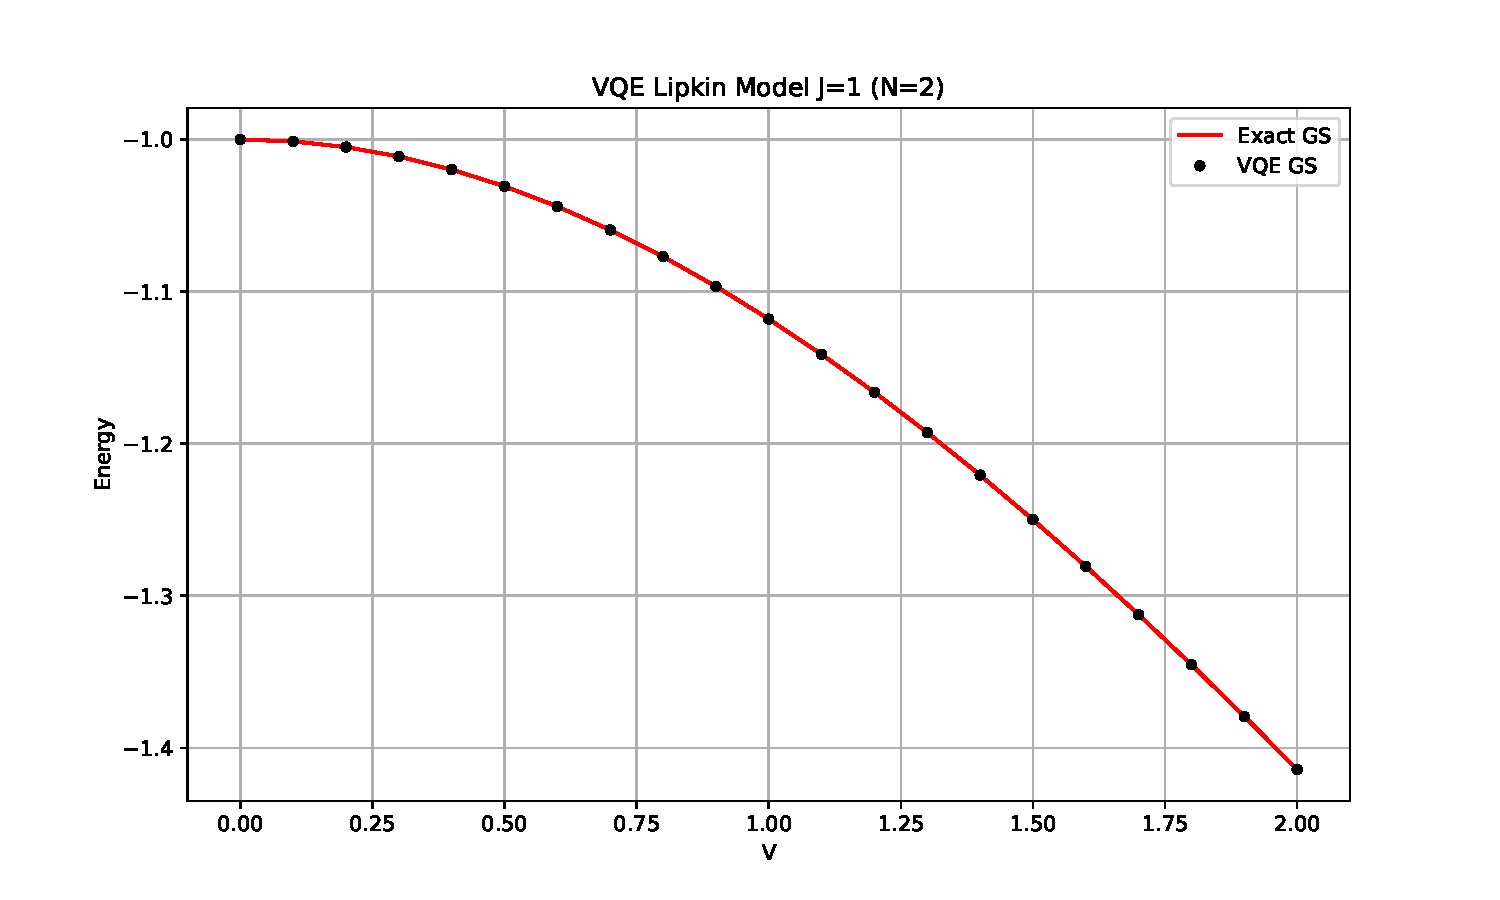
\includegraphics[width=0.55\linewidth]{figures/part-g_vqe_j1.pdf}
    \caption{VQE optimization landscape under variation of $J_1$ (Part G).}
    \label{fig:partg_vqe_j1}
\end{figure}
\end{document}





%%%%%%%%%%%%
\subsection{Part D methods}

\begin{equation}
    \ket{0}_{A,B} = [1\quad0]^T \quad \ket{1}_{A,B}=[0\quad1]^T
\end{equation}
\begin{equation}
    \ket{00}=\ket{0}_A\otimes\ket{0}_B=[1\quad0\quad0\quad0]^T
\end{equation}
\begin{equation}
    \ket{01}=\ket{0}_A\otimes\ket{1}_B=[0\quad1\quad0\quad0]^T
\end{equation}
\begin{equation}
    \ket{10}=\ket{1}_A\otimes\ket{0}_B=[0\quad0\quad1\quad0]^T
\end{equation}
\begin{equation}
    \ket{11}=\ket{1}_A\otimes\ket{1}_B=[0\quad0\quad0\quad1]^T
\end{equation}

\begin{equation}
    H_0\ket{00} = \epsilon_{00}\ket{00}
\end{equation}
\begin{equation}
    H_0\ket{10} = \epsilon_{10}\ket{10}
\end{equation}
\begin{equation}
    H_0\ket{01} = \epsilon_{01}\ket{01}
\end{equation}
\begin{equation}
    H_0\ket{11} = \epsilon_{11}\ket{11}
\end{equation}

\begin{equation}
    H_I=H_x\sigma_x\otimes\sigma_x+H_z\sigma_z\otimes\sigma_z
\end{equation}

\begin{equation}
    \mathbf{H} = \begin{bmatrix}
        \epsilon_{00}+H_z & 0 & 0 & H_x \\
        0 & \epsilon_{10}-H_z & H_x & 0 \\
        0 & H_x & \epsilon_{01}-H_z & 0 \\
        H_x & 0 & 0 & \epsilon_{11}+H_z
    \end{bmatrix}
\end{equation}

\begin{equation}
    \rho_0 = 
    (\alpha_{00}\ket{00}\bra{00} + 
    \alpha_{10}\ket{10}\bra{10} +
    \alpha_{01}\ket{01}\bra{01} +
    \alpha_{11}\ket{11}\bra{11})
\end{equation}
\begin{equation}
    \rho_A=\text{Tr}_B(\rho_0)=\bra{0}\rho_0\ket{0}_B+\bra{1}\rho_0\ket{1}_B
\end{equation}
\begin{equation}
    \rho_B=\text{Tr}_A(\rho_0)=\bra{0}\rho_0\ket{0}_A+\bra{1}\rho_0\ket{1}_A
\end{equation}
\begin{equation}
    S(A,B)=-\text{Tr}(\rho_{A,B}\log_2(\rho_{A,B}))
\end{equation}

\subsection{Part E methods}

\texttt{Qiskit} and \texttt{Pennylane}

\subsection{Part F methods}

$H=H_0+H_1+H_2$

\begin{equation}
    H_0=\frac{1}{2}\varepsilon\sum_{p\sigma}\sigma a_{p\sigma}^{\dagger}a_{p\sigma}
\end{equation}

\begin{equation}
    H_1=\frac{1}{2}V\sum_{p,p',\sigma}\sigma a_{p\sigma}^{\dagger}a_{p\sigma}
\end{equation}

\begin{equation}
    H_2=\frac{1}{2}W\sum_{p,p',\sigma}a_{p\sigma}^{\dagger}a_{p'\sigma}^{\dagger}a_{p'-\sigma}a_{p-\sigma}
\end{equation}

\begin{equation}
    H_0=\varepsilon J_z
\end{equation}

\begin{equation}
    H_1=\frac{1}{2}V(J_+^2+J_-^2)
\end{equation}

\begin{equation}
    H_2=\frac{1}{2}W(-N+J_+J_-+J_-J_+)
\end{equation}

\begin{equation}
    H_{J=1} = \begin{pmatrix}
        -\epsilon & 0 & -V \\
        0 & 0 & 0 \\
        -V & 0 & \epsilon
    \end{pmatrix}
\end{equation}

For $J=2$ we have a $5\times5$ matrix given by

\begin{equation}
    H_{J=2}=\begin{pmatrix}
        -2\epsilon & 0 & \sqrt{6}V & 0 & 0 \\
        0 & -\epsilon + 3W  & 0 & 3V & 0 \\
        \sqrt{6}V & 0 & 4W & 0 & \sqrt{6}V \\
        0 & 3V & 0 & \epsilon+3W & 0 \\
        0 & 0& \sqrt{6}V & 0 & 2\varepsilon
    \end{pmatrix}
\end{equation}

\subsection{Part G methods}




%%%%%%%%% RESULT



% \subsection{Part A results}

% \subsection{Part B results}

% \begin{lstlisting}[caption={VQE solver loop},label={lst:vqe-loop}]
% # Solve for lambda in [0, 1]
% lambdas = np.linspace(0, 1, 101)
% eigvals = []
% eigvecs = []

% for l in lambdas:
%     H = H0 + l * HI
%     w, v = np.linalg.eigh(H)
%     eigvals.append(w)
%     eigvecs.append(v)

% eigvals = np.array(eigvals)
% eigvecs = np.array(eigvecs)
% \end{lstlisting}

% \subsection{Part C results}

% \begin{equation}
%     E_1=0.0
%     \quad
%     E_2 = 4.0
% \end{equation}
% \begin{equation}
%     V_{11} = 3.0 \quad V_{12} = 0.2
% \end{equation}
% \begin{equation}
%     V_{21} = 0.2 \quad V_{22} = -3.0
% \end{equation}
% \begin{equation}
%     H_0=\begin{pmatrix}
%         E_1&0\\0&E_2
%     \end{pmatrix}
%     =\begin{pmatrix}
%         0&0\\0&4
%     \end{pmatrix}
% \end{equation}
% \begin{equation}
%     H_I = \begin{pmatrix}
%         V_{11} & V_{12} \\
%         V_{21} & V_{22}
%     \end{pmatrix}
%     =\begin{pmatrix}
%         3.0 & 0.2 \\
%         0.2 & -3.0
%     \end{pmatrix}
% \end{equation}

% \begin{equation}
%     \mathcal{E} = 2.0 \quad \Omega=-2.0 \quad \omega_z=3.0 \quad \omega_x=0.2
% \end{equation}

% \begin{equation}
%     H(\lambda)=H_0+\lambda H_1
% \end{equation}

% \begin{equation}
%     H(\lambda)\mathbf{v}_i=E_i(\lambda)\mathbf{v}_i
% \end{equation}

% \begin{equation}
%     H(\lambda)=\varepsilon\textbf{I}+(\lambda\omega_z+\Omega)\sigma_z+(\lambda\omega_x)\sigma_x
% \end{equation}

% \begin{equation}
%     \ket{\psi(\theta)} = R_y(\theta)\ket{0}
% \end{equation}

% \begin{equation}
%     \ket{\psi(\theta)} = \begin{pmatrix}
%         \cos\left(\frac{\theta}{2}\right) \\ \sin\left(\frac{\theta}{2}\right)
%     \end{pmatrix}
% \end{equation}

% \begin{equation}
%     \langle\sigma_z\rangle=\cos(\theta) 
%     \quad
%     \langle\sigma_x\rangle=\sin(\theta)
% \end{equation}

% \begin{equation}
%     E(\theta,\lambda) = \varepsilon+(\lambda\omega_z+\Omega)\cos(\theta)+(\lambda\omega_x)\sin(\theta)
% \end{equation}

% \begin{equation}
%     E_{\text{VQE}}(\lambda)=\min_{\theta}E(\theta,\lambda)
% \end{equation}
% \begin{equation}
%     E_{\text{exact}}(\lambda)
% \end{equation}

% \begin{equation}
%     \lambda_i\in[0,1] \quad i=1,\dots,51 
% \end{equation}

% \subsection{Part D results}

% \begin{equation}
%     H_x=2.0 \quad H_z=3.0
% \end{equation}

% \begin{equation}
%     \ket{\epsilon}_{00} = 0.0 \quad \ket{\epsilon}_{10} = 2.5
% \end{equation}
% \begin{equation}
%     \ket{\epsilon}_{01} = 6.5 \quad \ket{\epsilon}_{11} = 7.0
% \end{equation}


% \subsection{Part E results}
% \subsection{Part F results}
% \subsection{Part G results}
